\documentclass[14pt]{beamer}

\mode<presentation> {
\usetheme{Madrid}

% To remove the navigation symbols from the bottom of all slides uncomment next line
\setbeamertemplate{navigation symbols}{} 
\date{}
\title{}
\author{}

%to get rid of footer entirely uncomment next line
\setbeamertemplate{footline}{}
}


\usepackage{geometry}
\usepackage{multirow}
\usepackage{adjustbox}
\usepackage{multicol}
\setlength{\columnsep}{0.1cm}



\usepackage{tikz}
\usetikzlibrary{shapes,backgrounds}

\usepackage{bbding}
\usepackage{rotating}
\usepackage{xcolor}


%\usepackage{tkz-berge} %cool grid
\usepackage{pgfplots} %pics

\usepackage{graphicx} % Allows including images
\usepackage{booktabs} % Allows the use of \toprule, \midrule and \bottomrule in tables
\usepackage{mathtools}

\newcommand {\DS} [1] {${\displaystyle #1}$}
\newcommand {\R}{\mathbb{R}}
\newcommand {\Z}{\mathbb{Z}}
\newcommand {\N}{\mathbb{N}}
\newcommand{\e}{\varepsilon}

\newcommand{\p}{\pause}

% simple environrment for enumerate, easier to read
\setbeamertemplate{enumerate items}[default]

%%%%%%%%%%%%%%%%%%%%%%

% to use colours easily
\definecolor{miverde}{rgb}{0.7, .5, 0.7}
\newcommand{\azul}[1]{{\color{blue} #1}}
\newcommand{\rojo}[1]{{\color{red} #1}}
\newcommand{\verde}[1]{{\color{miverde} #1}}
 
% box in red and blue in math and outside of math
\newcommand{\cajar}[1]{\boxed{\mbox{\rojo{ #1}}}}
\newcommand{\majar}[1]{\boxed{\rojo{ #1}}}
\newcommand{\cajab}[1]{\boxed{\mbox{\azul{ #1}}}}
\newcommand{\majab}[1]{\boxed{\azul{ #1}}}
 
\newcommand{\setsize}[1]{\fontsize{#1}{#1}\selectfont} %allows you to change the font size. The default size of this document is 14. To change the font size of the whole slide, place this at the beginning of the slide. To change the size of only a portion of the text to size 12, you can do the following { \setsize{12} Your text. }.

\setbeamerfont{frametitle}{size=\setsize{15}}
\setbeamerfont{block title}{size=\setsize{14}}

\newcommand{\smallerfont}{\setsize{13}} %place this at the beginning of a slide to set the font size of the entire slide to 13.

%===========================
% Preamble just for this file
%===========================

\newcommand{\arcsec}{\operatorname{arcsec}}

\setbeamertemplate{enumerate items}{(\Alph{enumi})}
%===================================================
\begin{document}
%===================================================


\begin{frame}
	\frametitle{MAT137 Lecture 22 --- Inverse Functions}

	\vfill
	{\bf Before next class:}
		\begin{itemize} \normalsize
			\item {\bf Watch videos  4.3, 4.4}
		\end{itemize}
\end{frame}

\begin{frame}[t]
\frametitle{Worm up}

% Why this question?  Some students will answer ``False" because ``the graph crosses itself"


A worm is crawling accross the table.  The path of the worm looks something like this:

%\vspace{-1cm}

	\begin{center}
		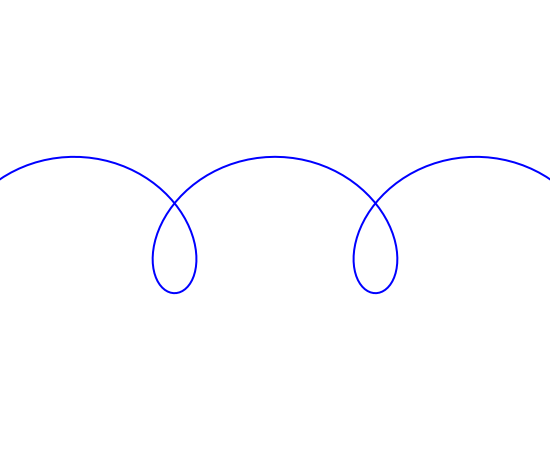
\includegraphics[scale=.3]{G11}
	\end{center}

\vspace{-1cm}

\begin{block}{True or False?}
The position of the worm is a function.
\end{block}

\end{frame}

%-----------------------------
\begin{frame}[t]
\frametitle{Worm function}


\vspace{-.7cm}

	\begin{center}
		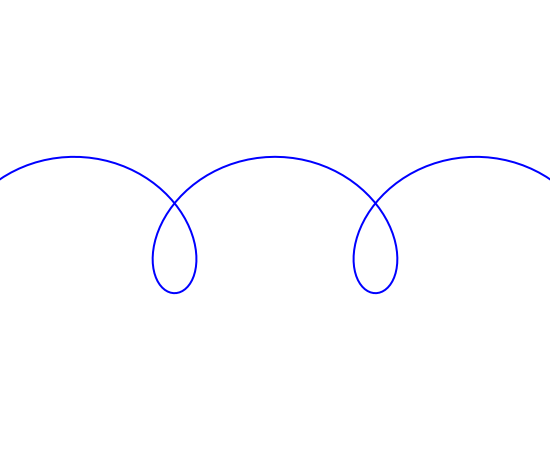
\includegraphics[scale=.3]{G11}
	\end{center}

\vspace{-1.5cm}

A worm is crawling accross the table.   \\
For any time $t$, let $f(t)$ be the position of the worm.  \\
This defines a function $f$.

\begin{enumerate}
	\item  What is the domain of $f$?
	\item  What is the codomain of $f$?
	\item  What is the range of $f$?
\end{enumerate}

\end{frame}

\begin{frame}[t]
\frametitle{Function, number, or nonsense?}

Let $f,g$ be functions. Let $x$ be a number. Classify each
	expression as a \textbf{function}, \textbf{number}, or \textbf{nonsense}.


\begin{multicols}{2}
	\begin{enumerate}
		\item $f(x)$
		\item $f\circ g$
		\item $f\circ (g(x))$
		\item $(f\circ g)(x)$
		\item $f(x)\circ g(x)$
		\item $f(x)g(x)$
		\item $f(g(x))$
		\item $f(g)$
		\item $f(g)(x)$
		\item $f(g(x)f(x))$
		\item $e^x$
		\item $\ln x$
		\item $\ln$
		\item $\sin \circ e^x$
		\item $\sin \circ \ln$
		\item $(\ln\circ \sin)(e^x)$
		\item $e^x\circ \sin$
		\item $\sin^2$
	\end{enumerate}
\end{multicols}


\end{frame}

\begin{frame}
\frametitle{Inverse function from a graph}

\begin{columns}[c]

\column{.65\textwidth}
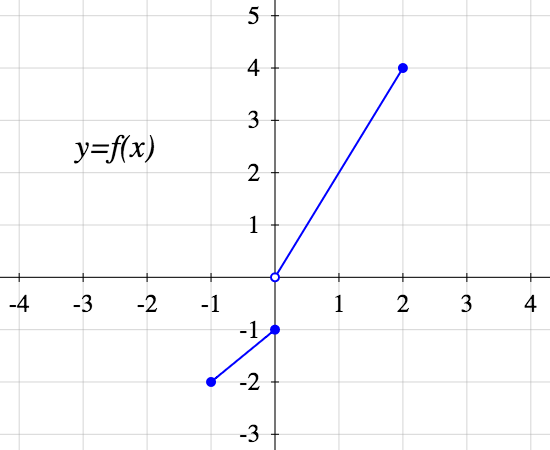
\includegraphics[scale=.4]{G12}
\column{.3\textwidth}
Calculate:
\begin{enumerate}
	\item  \DS{f(2)}
	\item  \DS{f(0)}
	\item  \DS{f^{-1}(2)}
	\item  \DS{f^{-1}(0)}
	\item  \DS{f^{-1}(-1)}
\end{enumerate}
\end{columns}

\end{frame}

\begin{frame}[t]
\frametitle{Absolute value and inverses}

Let
	$$
		h(x) = x |x| + 1
	$$
\begin{enumerate}
	\item  Calculate \DS{h^{-1}(-8)}.
\p
	\item Sketch the graph of $h$.
	\item  Find an equation for \DS{h^{-1}}.
	\item Sketch the graph of \DS{h^{-1}}.
	\item  Verify that
		\begin{itemize} \normalsize
			\item  for every \DS{t \in \boxed{???}}, \; \DS{h(h^{-1}(t)) = t}.
			\item for every \DS{t \in \boxed{???}}, \; \DS{h^{-1}(h(t)) = t}.
		\end{itemize}
\end{enumerate}

\end{frame}



\begin{frame}[t]
\frametitle{Composition and inverses}

Assume for simplicity that all functions in this problem have domain $\R$.

\vfill

Let $f$ and $g$ be functions.  Assume they each have an inverse.

\vfill

Is \DS{\left( f \circ g \right)^{-1} = f^{-1} \circ g^{-1}}?

\begin{itemize}
	\item If YES, prove it. 
	\item If NO, fix the statement.
\end{itemize}


\vfill  \p

If you do not know how to start, experiment with the functions
	$$
		f(x) = x + 1, \quad \quad g(x) = 2x.
	$$

\end{frame}
















\begin{frame}
	\frametitle{MAT137 Lecture 23 --- Inverse Functions II}

	{\bf Warmup:}

	$f$ is defined so that for $t\in\mathbb R$, we have $f(t)=(|t|,-|t|)$.

	$g$ is defined so that for $t\in\mathbb R$, we have $g(t)=\pm |t|$.

	\medskip

	For each of $f$ and $g$, find a domain/codomain such that they are a function,
	or explain why you can't.

	\vfill
	{\bf Before next class:}
		\begin{itemize} \normalsize
			\item {\bf Watch videos 4.5, 4.7, 4.8, 4.9 }
		\end{itemize}
\end{frame}


\begin{frame}
\frametitle{Fill in the Blank }

Given that $f$ is an invertible function, fill in the blanks. 
\begin{enumerate}
\item If $f(-1) = 0$, then $f^{-1}(0) =$ ------.
\item If $f^{-1}(2) = 1$, then $f(1)=$ ------.
\item If $(2,3)$ is on the graph of $f$, then ------  is on the graph of $f^{-1}$.
\item If ------ is on the graph of $f$, then $(-2,4)$ is on the graph of $f^{-1}$.
\end{enumerate}


\end{frame}

%-----------------------------
\begin{frame}[t]
\frametitle{Where is the error?}

	\begin{itemize}
		\item We know that \majab{(f^{-1})' = \frac{1}{f'}}
		\item  Let \DS{f(x) = x^2}, restricted to the domain \DS{x \in (0, \infty)}
			$$f'(x) = 2x \quad \mbox{and} \quad \majar{f'(4) = 8}$$
		\item  Then \DS{f^{-1}(x) = \sqrt{x}}
			$$(f^{-1})'(x) = \frac{1}{2\sqrt{x}} \quad \mbox{ and } \quad \majar{(f^{-1})'(4) = \frac{1}{4}}$$
		\item So \majab{(f^{-1})'(4) \neq \frac{1}{f'(4)}}
	\end{itemize}


\end{frame}

\begin{frame}[t]
\frametitle{Derivatives of the inverse function}


Let $f$ be a one-to-one function. \\
Let $a, b \in \R$ such that $b=f(a)$.

\vfill
\begin{enumerate}
	\item Obtain a formula for \DS{ \left(f^{-1}\right)'(b) } in terms of \DS{f'(a)}.
		\vspace{.2cm}
		
		{\smallerfont
		\emph{Hint:} This was done in Video 4.4  \\
		Take \DS{\frac{d}{dy}} of both sides of  \quad \DS{ f(f^{-1}( (y)) = y }.
		}
	
	 \vfill
	\item  Obtain a formula for \DS{ \left(f^{-1}\right)''(b) } in terms of \DS{f'(a)} and \DS{f''(a)}.

	 \vfill	
	\item   \emph{Challenge:}  Obtain a formula for \DS{ \left(f^{-1}\right)'''(b) } in terms of \DS{f'(a)}, \DS{f''(a)}, and \DS{f'''(a)}.

\end{enumerate}


\end{frame}

\begin{frame}[t]
\frametitle{Composition of one-to-one functions}


Assume for simplicity that all functions in this problem have domain $\R$.  Prove the following theorem.

\vfill


\begin{block}{Theorem A}
Let $f$ and $g$ be functions. \\
IF $f$ and $g$ are one-to-one, \\
THEN $f \circ g$ is one-to-one.
\end{block}

\vfill

Suggestion:
	\begin{enumerate}
		\item Write the definition of what you want to prove.

		\item  Figure out the formal structure of the proof.

		\item   Complete the proof (use the hypotheses!)
	\end{enumerate}

\end{frame}













\begin{frame}
	\frametitle{MAT137 Lecture 24 --- Exponentials and Logarithms}

	\vfill
	{\bf Before next class:}
		\begin{itemize} \normalsize
			\item {\bf Watch videos  4.12, 4.13, 4.14}
		\end{itemize}
\end{frame}


\begin{frame}[t]
\frametitle{Computations - Exponentials and logarithms}



Compute the derivative of the following functions:

\begin{enumerate}
	\item  \DS{f(x) = e^{\sin x + \cos x} \ln x}
\vfill
	\item  \DS{f(x) = \pi^{\tan x}}
\vfill
	\item  \DS{f(x) = \ln \left[ e^x + \ln  \ln  \ln x  \right]}
\vfill
	\item \DS{f(x) = \log_{10} \left( 2x + 3 \right)}
\vfill
\end{enumerate}


\end{frame}

\begin{frame}[t]
\frametitle{Logarithm and Absolute Value}

The function $F$ is defined by the equation
	$$F(x) = \ln |x| .$$
What is its derivative?
\vfill
	\begin{enumerate}
		\item  \DS{F'(x) = \frac{1}{x}}
\vfill
		\item  \DS{F'(x) = \frac{1}{|x|}}
\vfill
		\item  $F$ is not differentiable
\vfill
	\end{enumerate}
\end{frame}

\begin{frame}[t]
\frametitle{Logarithmic differentiation}

\vspace{5mm} 
	\begin{block}{}
Calculate the derivative of 
	$$
		g(x)  = x^{\tan x}.
	$$
	\end{block}

\end{frame}


%-----------------------------
\begin{frame}[t]
\smallerfont
\frametitle{More logarithmic differentiation}

\begin{block}{}
Calculate the derivative of 
	$$
		f(x) = \left( \sin x \right)^{\cos x} + \left( \cos x \right)^{\sin x}.
	$$
\end{block}


\pause \vfill

{\bf \underline{What is wrong with this answer?}}
	\begin{align*}
		\ln f(x)  = & (\cos x) \ln ( \sin x )+ ( \sin x ) ( \ln \cos x ) \\
		{\color{red} \frac{d}{dx}} \left[  \ln f(x) \right]  = & {\color{red} \frac{d}{dx}} \left[ (\cos x) \ln ( \sin x ) \right] + 
			 {\color{red} \frac{d}{dx}} \left[ ( \sin x ) ( \ln \cos x ) \right] \\
		\frac{f'(x)}{f(x)}  = & - ( \sin x ) \ln (\sin x) + (\cos x ) \frac{\cos x}{\sin x}  \\
				& + ( \cos x ) \ln (\cos x) + (\sin x ) \frac{- \sin x}{\cos x}
	\end{align*}
	$${f'(x) = f(x) \left[ - (\sin x) \ln(\sin x) + (\cos x) \ln (\cos x) + \frac{\cos^2 x}{\sin x} - \frac{\sin^2 x}{\cos x} \right]}$$
\end{frame}


\begin{frame}[t]
\frametitle{Cue Boss Music}

\vspace{5mm} 
\begin{block}{}
Calculate the derivative of 
	$$
		h(x) = \sqrt[3]{\frac{\left( \sin^6 x \right) \sqrt{x^7+6x+2}}{3^x \left(x^{10}+2x\right)^{10}}}
	$$
\end{block}


\end{frame}










\begin{frame}
	\frametitle{MAT137 Lecture 25 --- Inverse Trig}

	\vfill
	{\bf Before next class:}
		\begin{itemize} \normalsize
			\item {\bf Watch videos  5.2, 5.3, 5.4}
		\end{itemize}
\end{frame}

\begin{frame}[t]
\smallerfont
\frametitle{Definition of $\arctan$}

\begin{enumerate}
	\item  Sketch the graph of $\tan$.
	\item  Prove that $\tan$ is not one-to-one.
	\item  Select the largest interval containing $0$ such that the restriction of $\tan$ to it is one-to-one.
		We define $\arctan$ as the inverse of this restriction.  \quad Let $x, y \in \R$
%	\item 
		$$\arctan y = x \; \quad \; \iff \; \quad ???$$
	\item	What is the domain of \DS{\arctan}? 
		What is the range of \DS{\arctan}?
	
	 Sketch the graph of $\arctan$.
	\item Compute
		\begin{multicols}{2}
			\begin{enumerate}
				\item  \DS{\arctan \left( \tan \left( 1 \right) \right) }
				\item  \DS{\arctan \left( \tan \left( 3\right) \right) }
				\item \DS{\arctan \left( \tan \left( \frac{\pi}{2}\right) \right) }
				\item  \DS{\arctan \left( \tan \left( -6)\right) \right) }
				\item \DS{\tan \left( \arctan \left( 0\right) \right) }
				\item \DS{\tan \left( \arctan \left( 10\right) \right) }
			\end{enumerate}		
		\end{multicols}
\end{enumerate}



\end{frame}

\begin{frame}[t]
\frametitle{Trig-inverse-trig}

\begin{block}{}
Find simple expressions for these quantities and state the domain on which they are valid:
	\begin{enumerate}
	\begin{multicols}{2}
		\item  \DS{\sin \; ( \arccos x)}
		\item \DS{\sec \; (\arccos x)}
		\item \DS{\sec \; ( \arctan x)}
		\item \DS{\tan \; (\arcsec x)}
	\end{multicols}
	\end{enumerate}
\vspace{-.1cm}	
\end{block}

\ \p

{\smallerfont
\emph{Hint:}  There are two standard ways to attack these problems:
	\begin{itemize}
		\item  Use a trig identity  \\  e.g.: a trig identity relating $\sin$ and $\cos$ for (1)
		\item  Or draw a right triangle with side lengths $1$ and $x$ 
			\\ e.g.: with an angle $\theta$ such that $\cos \theta = x$ for (1)
	\end{itemize}
If you need to take a square root, you must justify which branch ($+$ or $-$) you are choosing.
}

\end{frame}



\begin{frame}[t]
\frametitle{A different type of logarithm}

Calculate the derivative of 
	$$
		f(x) = \log_{x+1} (x^2+1)
	$$
	
\vfill

\emph{Note:}  This is a new function.  We have not given you a formula for it yet,  That is on purpose.

\vfill \p

\emph{Hint:}  If you do not know where to start, remember the definition of logarithm:
	$$
	\log_a b = c \; \iff \; a^c = b.
	$$
	

\end{frame}
















%----------------------------------------------------------------------------------------
%	Functions and inverse functions
%----------------------------------------------------------------------------------------
%-----------------------------


%-----------------------------

\begin{frame}

\frametitle{\small Finding a Restricted Domain on which a Function is Invertible}
\vspace{-3mm}
%\begin{minipage}{0.35\textwidth}
\begin{center}
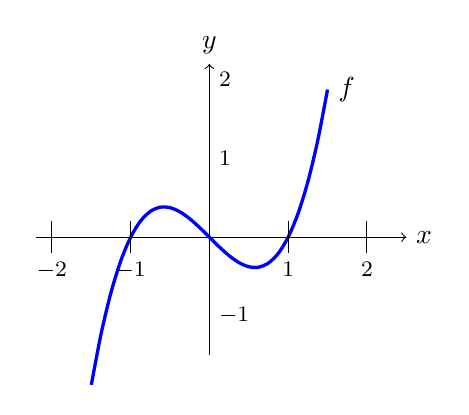
\begin{tikzpicture}[scale=1]
			\draw[->] (-2.2,0) -- (2.5,0) node[right] {$x$};
			\draw[->] (0,-1.5) -- (0,2.2) node[above] {$y$};
			\draw[draw= blue, very thick, scale=1,domain=-1.5:1.5,smooth,variable=\x] plot (\x,\x*\x*\x-\x) node[right] {$f$};
			
\node [below] at (-2,-0.2) {\footnotesize $-2$};
\node [below] at (-1,-0.2) {\footnotesize$-1$};
%\node [below] at (0,0) {\footnotesize$0$};
\node [below] at (1,-0.2) {\footnotesize$1$};
\node [below] at (2,-0.2) {\footnotesize$2$};
%

%\node [right] at (0,-2) {\footnotesize$-2$};
\node [right] at (0,-1) {\footnotesize$-1$};
\node [right] at (0,1) {\footnotesize$1$};
\node [right] at (0,2) {\footnotesize$2$};

			\draw(1,-0.2) -- (1,0.2);
			\draw(2,-0.2) -- (2,0.2);
			\draw(-1,-0.2) -- (-1,0.2);
			\draw(-2,-0.2) -- (-2,0.2);


		\end{tikzpicture}
		\end{center}
%		\end{minipage}
%		%%%%%%%%
%\begin{minipage}{0.6\textwidth}
\begin{enumerate}
\item Find the largest interval containing 0 on which $f$ is invertible.
\item Find the largest interval containing 1 on which $f$ is invertible.
\end{enumerate}


\end{frame}


%-----------------------------


%-----------------------------

%-----------------------------
%-----------------------------
\begin{frame}[t]
\frametitle{Functions, inverses, and graphs }

Sketch the graph of a function $g$ satisfying all the following properties:

\begin{enumerate}
	\item  The domain of $g$ is $\R$.
	\item $g$ is continuous everywhere except at $-2$.
	\item $g$ is differentiable everywhere except at $-2$ and $1$.
	\item  $g$ has an inverse function.
	\item  $g(0)=2$
	\item $g'(0) = 2$
	\item \DS{\left(g^{-1}\right)' (-3) = -2}.
\end{enumerate}

\end{frame}

%-----------------------------
\begin{frame}[t]
\frametitle{Functions, inverses, and graphs - 2}
%This appeared in a past test

Draw the graph of a function $f$ satisfying all of the following:

	\begin{enumerate}
		\item The domain of $f$ is $\R$.
		\item $f$ is differentiable everywhere.
		\item The restriction of $f$ to \DS{[0, \infty)} is one-to-one,  \\ and its INVERSE has a vertical tangent line at $2$.
		\item The restriction of $f$ to \DS{(- \infty,0]} is one-to-one,  \\ and its INVERSE has derivative $2$ at $2$.
	\end{enumerate}

\end{frame}
%-----------------------------
%-----------------------------

%-----------------------------
\begin{frame}[t]
\frametitle{Composition of one-to-one functions -- 2}

Assume for simplicity that all functions in this problem have domain $\R$.   Prove the following theorem.


\begin{block}{Theorem B}
Let $f$ and $g$ be functions. \\
IF $f \circ g$ is one-to-one, \quad
THEN $g$ is one-to-one.
\end{block}


\p
Suggestion:
	\begin{enumerate}
		\item  Transform the ``\DS{P \implies Q}'' theorem into an equivalent 
		``\DS{\mbox{(not Q)} \implies \mbox{(not P)} }'' theorem.  \\ You will prove that one instead.
\p
		\item Write the definition of the hypotheses \\ and of the conclusion.

		\item Write the proof.
	\end{enumerate}

\end{frame}
%-----------------------------
\begin{frame}[t]
\frametitle{Composition of one-to-one functions -- 3}

Assume for simplicity that all functions in this problem have domain $\R$.

\vfill

Prove the following claim is FALSE with a counterexample.

\vfill


\begin{block}{Claim }
Let $f$ and $g$ be functions. \\
IF $f \circ g$ is one-to-one, \\
THEN $f$ is one-to-one.
\end{block}

\vfill

\end{frame}

%----------------------------
\begin{frame}[t]
\frametitle{Increasing and one-to-one}

\begin{block}{Definition}
Let $f$ be a function with domain $D$. We say that $f$ is \emph{increasing} on $D$ when

$$\forall x_1, x_2 \in D,  \quad x_1<x_2 \implies f(x_1)<f(x_2).
$$
\end{block}

\begin{enumerate}
\item Prove that if a function is increasing, then it is one-to-one.
\p
\item Use this to show that $g(x) = x^5 + 4x^3 + 2x + 1$ has an inverse.
\item Find $(g ^{-1})'(1)$.
\end{enumerate}


\end{frame}

%-----------------------------
%----------------------------------------------------------------------------------------
%	Exponentials and logarithms
%----------------------------------------------------------------------------------------
%-----------------------------
%-----------------------------
%-----------------------------
%-----------------------------
%-----------------------------

%-----------------------------
\begin{frame}[t]
\frametitle{An Implicit Function}

\vspace{5mm} 
\begin{block}{}
Find $y'$ if $x^y=y^x$.
\end{block}
\end{frame}


%-----------------------------
%----------------------------------------------------------------------------------------
%	Inverse trig functions
%----------------------------------------------------------------------------------------
%-----------------------------

%-----------------------------
\begin{frame}[t]
\frametitle{Derivative of $\arctan$}

\begin{block}{}
Obtain (and prove) a formula for the derivative of $\arctan$.
\end{block}

\

\emph{Hint:}  Call \DS{f(t) = \arctan t} and differentiate
	$$
		\forall t \in \ldots \quad \quad \tan ( f(t)) = t
	$$
\end{frame}
%-----------------------------
\begin{frame}[t]
\frametitle{Computations - Inverse trig functions}


Compute the derivatives of these functions, and simplify them as much as possible:
	\begin{enumerate}
		\item  \DS{f(x) = \arcsin \left( x^{3/2}\right) }
		\vfill
		\item  \DS{ f(x)=2x^2 \arctan (x^2) - \ln (x^4+1) }
		\vfill
	\end{enumerate}

\end{frame}

%-----------------------------
%-----------------------------
\begin{frame}[t]
\frametitle{$\arcsec$}


\begin{enumerate}

\item  Complete: ``We define $\arcsec$ as the inverse of 
 the restriction of $\sec$ to ..."

\emph{Hint:} Sketch the graph of $\sec$.  

\vfill

\item What are the domain and range of $\arcsec$?  \\ Sketch its graph.

\vfill

\item Obtain (and prove) a formula for the derivative of $\arcsec$ in the same way you did for $\arctan$.

\vfill

\item Now obtain the same formula  in a different way:  use \DS{\sec x = \frac{1}{\cos x}} to write \DS{\arcsec} in terms of \DS{\arccos}.

\end{enumerate}


\end{frame}
%-----------------------------

%------------------------------
%-----------------------------
\end{document}
%-----------------------------
%-----------------------------









